\documentclass[main.tex]{subfiles}
\begin{document}
За да кажем как ще разпознаваме емоции в сигнали, трябва да изберем две неща. Първо, какво ще наричаме емоция и второ - кои емоции ще класифицираме.

Най-точното описание, което може да се даде за емоция, е може би цитатът на Потър Стюърд (член на Върховния съд на САЩ):  ``Когато го видя, ще го разпозная''\footnote{I know it when I see it}. Изкушаващо е да се използват за случая думите му: ``Няма днес да се опитвам точно да дефинирам материята, попадаща под това кратко описание; възможно е никога да не мога да дам разбираемо описание. Но едно нещо знам, когато го видя, ще го разпозная.''. За да можем да продължим напред в текста на дипломната работа обаче, ще трябва да работим с малко по-конкретни дефиниции.

Един от най-ранните опити да се дефинира емоция идва от Чарлз Дарвин и книгата му ``За изразяването на емоциите при човека и животните'' от 1872 г. 
Той използва емоцията, за да потвърди еволюционната си теория, тъй като според неговите наблюдения изразяването на емоциите е сходно между животните и хората и се обяснява еволюционно. В книгата си Дарвин представя три принципа, които описват изразяването на емоциите:
\begin{enumerate}
    \item ``Принцип на полезните навици''
    
    Такива са смръщване на вежди, при което в очите влиза по-малко светлина, или вдигане на вежди, което увеличава полето на зрение. Когато човек е учуден, той вдига вежди, за да ``види по-ясно ситуацията''. Такива навици, според Дарвин, се предават наследствено заради полезния си характер.
    \item ``Принцип на противоположностите''
    
    Това са навици, които нямат практическа полза, но представляват противоположност на някакъв друг естествен навик. Пример за това е свиването на рамене, което е израз противоположен на уверено или агресивно изразяване.
    
    \item ``Принцип на нервните сигнали''
    
    Когато се говори за Дарвиновата теория, най-често се има предвид този принцип. Според него, някои навици са породени от сигнал от нервната система. Такива са например изявите на гняв и страх.
\end{enumerate}

Тъй като тези изрази на емоция се предават еволюционно, то те се наблюдават у всички животни (в частност и хора). 

Тази представа за емоциите е продължена от Робърт Плутчик (1927 - 2006). Базирайки се на еволюционната теория, той се опитва да опише понятието ``емоция''. Наблюденията му в \cite{plut} са следните:

Еволюционният произход на някои емоции е по-явен от при други. Например изразът на страх при животните и хората е много сходен и цели едно и също - да премахне причинителя. Изразът на любов обикновено е с репрудукционни цели. Някои емоции обаче са по-сложни и първоизточникът им се описва по-трудно, затова търсим начин да генерализираме понятието. Емоцията е сложна верига от събития, която започва с някакъв стимул. В следствие настъпва фаза на ``изпитване на емоция'' и фаза на физиологични промени (тук възниква научният спор за кокошката и яйцето - дали чувството е първо или физиологичните промени). Те предизвикват целенасочено държание, което цели да премахне дразнението на стимула и да върне състоянието на еквилибриум. 

Плутчик прави психо-еволюционна класификация на емоциите, като избира осем главни емоции - две по две противоположни. Всяка от тези базови емоции е свързана с поведение, важно за оцеляването. Например страх и поведението "бий се или бягай", свързано с освобождаването на хормони, подготвящи организма за бягство или битка. Всяка от не-базовите емоции се получава като комбинация на базовите. Плутчик сравнява това с комбинирането на цветове, което може да се види и на известното му ``Колело на емоциите'' (1980), показано на \autoref{fig:emotions:1}.

\begin{minipage}{0.45\textwidth}
    \begin{figure}[H]%
        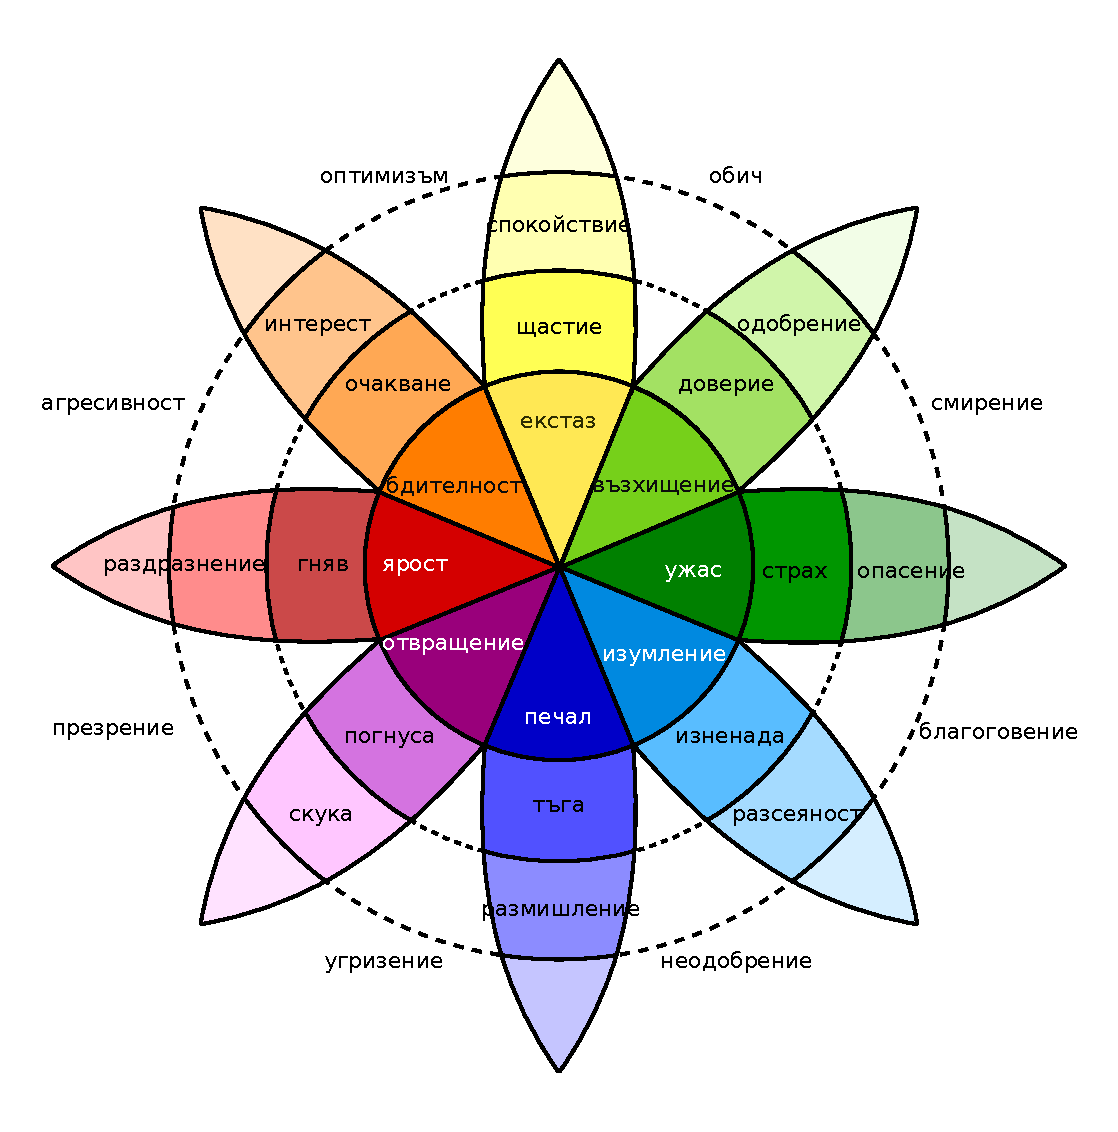
\includegraphics[width=\textwidth ]{plutchik}
        \caption{Колелото на емоциите на Плутчик}
        \label{fig:emotions:1}
    \end{figure}
\end{minipage} \hfill
\begin{minipage}{0.45\textwidth}
    Базовите емоции са: страх, изненада, тъга, погнуса, гняв, очакване, щастие, доверие. По ``листенцата'' на всяка от тях се намират по-силният и съответно по-слабият вариант. За съжаление, колкото повече класове искаме да класифицираме, толкова повече данни са нужни, което прави използването на класификацията на Плутчик трудно за практически цели. Друг проблем при голямото разнообразие на Плутчиковото колело е, че различните емоции имат различна продължителност на проявлението, като например тъгата може да продължава с дни, докато изпитването на погнуса е много по-моментно. Това прави съставянето на база данни за емоционално разпознаване трудно.
\end{minipage}

След като вече започнахме с цитат, време е и за другото клише, а именно етимология. Думата емоция произлиза от френското émouvoir (вълнувам, възбуждам интерес) и по-назад латинскоро ēmoveō (местя навън/извън пътя). Затова е и естествена класификацията на база как ``вълнува'' съответната емоция. Известна такава класификация е VAD моделът, разработен от Алберт Мейерабиан и Джеймс Ръсел \cite{pad}, в който всяка емоция се описва в тримерно пространство с оси ``валентност'', ``ниво на възбуда'', ``доминантност''\footnote{\textbf{V}alence, \textbf{A}rousal, \textbf{D}ominance}. Оста за валентност определя дали емоцията е приятна или не, оста за нивото на възбуда описва колко енергия е нужна за изразяването на емоцията, а доминантност - колко доминиращ или съответно пок\`{о}рен се чувства човек под влиянието на емоцията. По-често се използва опростен модел, наречен валентност-активация, който използва само две от осите (нивото на възбуда наричаме активация). Изразяването на някои емоции в този модел е показано на \autoref{fig:emotions:2}
\begin{figure}[ht]%
    \centering
    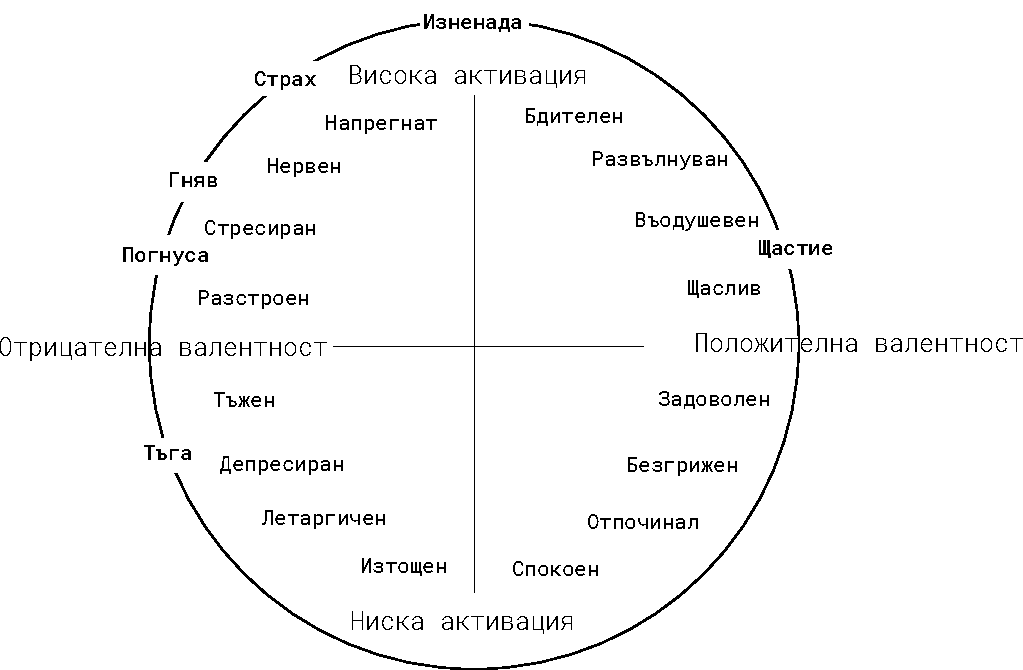
\includegraphics[width=\textwidth ]{valence_arousal}
    \caption{Модел ``валентност-аквитация''}
    \label{fig:emotions:2}
\end{figure}

За да изберем кои емоции да разпознаваме, нека разгледаме какви са силните и слабите страни на двете изследвани области.
Според \cite{survey}, в речта лесно се разпознават характеристики, свързани с активацията, тъй като нивото на активацията се отразява на енергията на говора. Тоест емоции като щастие и гняв (които са с висока активация) карат хората да говорят много по-силно и възбудено, докато емоции като тъга и умора (с ниска активация) са свързани с много по-пасивно поведение като цяло.
Дадените примери за разпознаване на емоциите в мозъка чрез ЕЕГ сигнал в \cite{brain_survey} показват, че по-лесно се разпознава валентност, макар че може да бъде извлечена информация и за активацията.

При избора на емоции, които да изследваме, трябва да изберем такива, за класификацията на които ще помогнат и двата сигнала - тоест да има примери в различните квадранти (ако е възможно) на VAD-модела. Тъй като основните емоции на Плутчик са твърде много, трябва да изберем тяхно подмножество. В случая ще разглеждаме четири емоции - три от които са част от базовите, а четвъртата емоция е ``неутрална емоция''. Изборът е такъв, че хем да нямаме прекалено много класове, хем тези емоции да могат да се предизвикват лесно в опитна среда и да могат да се описват вербално.
Финално избраните емоции, които ще се опитваме да разпознаваме в сигнали от реч и ЕЕГ, са следните:
\begin{enumerate}
    \item \textbf{Гняв} - висока активация, отрицателна валентност
    \item \textbf{Щастие} - висока активация, положителна валентност
    \item \textbf{Неутрална емоция} - неутрална активация, неутрална валентност
    \item \textbf{Тъга} - ниска активация, отрицателна валентност
\end{enumerate}

След този бегъл опит да дефинираме понятието емоция и да изберем кои класове емоции ще изследваме, трябва да разгледаме свойствата на двата входни сигнала. Нека започнем от сигналите от реч. 

\end{document}